\documentclass[ngerman]{article}

\usepackage[utf8]{inputenc}
\usepackage[ngerman]{babel}

\usepackage{listings}
\usepackage{color}
\usepackage{graphicx}

\author{Julius Adorf, Marek Kubica, Hong-Khoan Quach\\Technische Universität München}

\title{ETI-Großprojekt 8\\
       Sommersemester 2009\\
       {\bf Das Carrierpigeon-Projekt}
}

\date{\today}

% cheat a little bit
% code samples should not be split
\setlength{\headheight}{-20pt}
\setlength{\textheight}{590pt}

% colorize code samples
\lstset{language=C}
\lstset{
    basicstyle=\small,
    keywordstyle=\color[rgb]{0.1,0.1,0.8}
    }

\setlength{\parindent}{0cm}
\setlength{\parskip}{1em}

\begin{document}

\maketitle

\begin{abstract}

Das Carrierpigeon-Projekt ist ein studentisches Lernprojekt, dessen Ziel es
war, ein System zu erstellen, in dem man mit einem Handy mittels Bluetooth
Nachrichten an einen elektronischen Briefkasten senden kann. Auf dem
elektronischen Briefkasten kann man die empfangenen Nachrichten anzeigen und
anschließend auch löschen. Der Briefkasten besteht aus einem Mikrocontroller,
einer kleinen Flüssig\-kristall\-an\-zeige, einigen Tasten und einem
Bluetooth-Modul.

\end{abstract}

\section{Motivation}

Das Carrierpigeon-Projekt ist 2009 am Lehrstuhl für Rechnertechnik und
Rechnerorganisation der Technischen Universität München im Rahmen eines
studentischen Praktikums entstanden. Uns ging es darum, zu untersuchen, wie man
mit einem Mikrocontroller über Bluetooth mit Geräten in der Umgebung
kommunizieren kann, und zudem eine Anwendung zu entwickeln, die diese Form der
Kommunikation integriert. Es ging nicht darum, einen Prototypen für ein
markttaugliches System zu erstellen. Stattdessen stand der Lerneffekt und die
Lösung der technischen Fragestellungen im Vordergrund.

Trotzdem haben wir in der Entwicklung nicht nur experimentiert, sondern uns an
einer bestimmten Idee orientiert, um klare Anforderungen an das System zu
erhalten. Begonnen hat das Projekt mit folgenden Anwendungsfall:

\begin{quote}

Alpha möchte Beta besuchen. Beta ist leider nicht da. Daher möchte Alpha eine
Nachricht mit seinem Handy auf Betas elektronischen Briefkasten hinterlassen.
Kommt Beta nun zurück, so kann Beta sich die empfangenen Nachrichten
durchlesen.

\end{quote}

In dieser Projektbeschreibung geht es uns nicht darum, ein Referenzhandbuch zu
erstellen. Vielmehr möchten wir hier die Ideen hinter der Implementierung
vorstellen und die Konzepte beleuchten, die aus dem Quelltext nicht immer so
leicht erkennbar sind.

Dieses Dokument wurde aus Revision \\
\texttt{\input{current-hg-tip}} \\des
Carrierpigeon-Repositories erstellt.

\section{Begriffe}

In dem gerade beleuchteten Szenario treten verschiedene Rollen und technische
Komponenten auf. Die beiden technischen Komponenten sind der
\textit{Briefkasten} und das \textit{Mobiltelefon}. Der \textit{Sender} ist der
Benutzer, der vom Mobiltelefon aus Nachrichten sendet. Den Benutzer, an den die
Nachrichten adressiert sind und der diese lesen kann, nennen wir
\textit{Empfänger}.

Die Rollen des Senders stellen einige Anforderungen an das Programm auf dem
Mobiltelefon. Als Sender soll man auf einfache Art und Weise eine Nachricht
eingeben können. Als Sender soll man einen Briefkasten aus einer Liste wählen
und diesem eine Nachricht senden können.

Analog dazu legt die Rolle des Empfängers die Anforderungen an den Briefkasten
fest: Als Empfänger bekommt man die neueste Nachricht an\-gezeigt. Man soll
eine beliebige der gespeicherten Nachrichten anzeigen können. Schließlich soll
man als Empfänger gespeicherte Nachrichten löschen können.

\section{Architektur}

\subsection{Hardware-Architektur des Briefkastens}

Der Briefkasten besteht aus einem ATmega8515-Mikrocontroller, der über Ports,
die auf Register abgebildet werden, eine ST565-Flüssigkristallanzeige bedienen
kann. Der Mikrocontroller kann mit einen UART-Baustein -- also über eine serielle
Schnittstelle -- mit dem BTM-222-Bluetooth-Modul kommunizieren. Im Folgenden
gibt ein Schaubild eine grobe Übersicht der wichtigsten Hardware-Elemente. Für
eine genaue Spezifikation sei hier auf die Referenzhandbücher des ATmega8515,
des ST565 bzw. des BTM-222 verwiesen.

\begin{figure}[h!] \begin{center}
    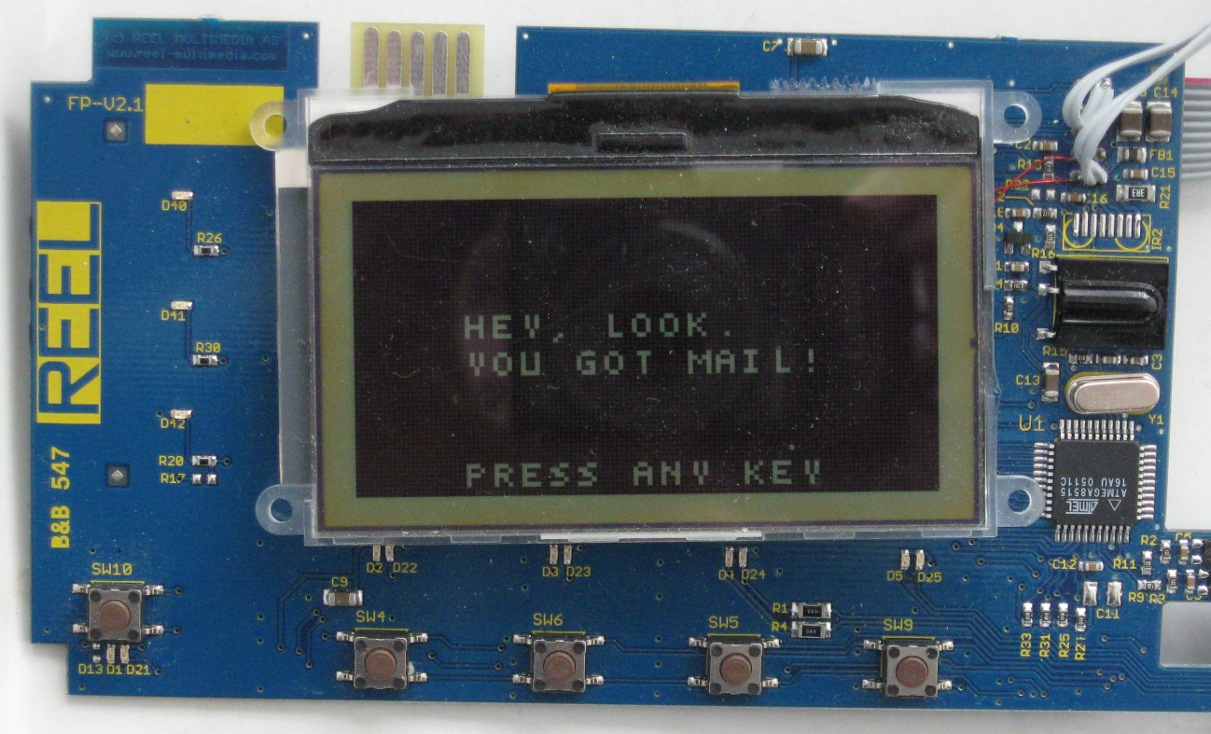
\includegraphics[width=0.5\textwidth]{media/board}
    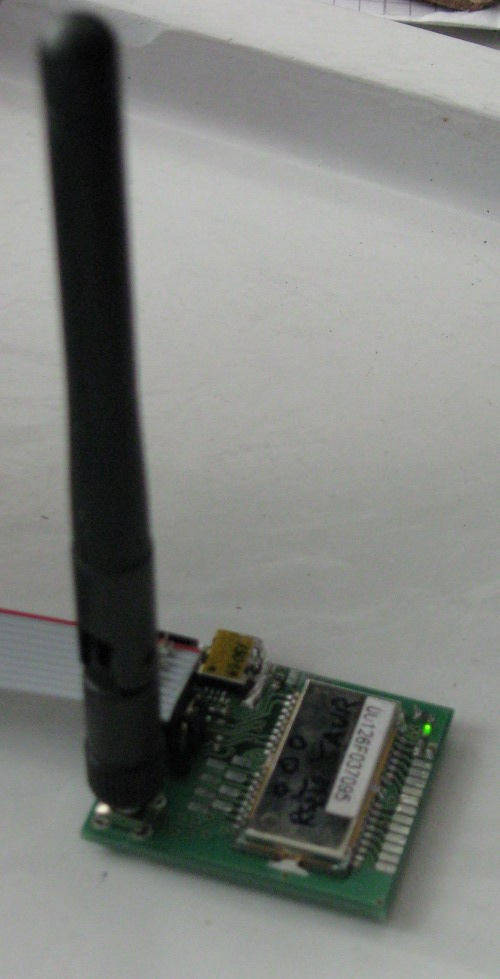
\includegraphics[width=0.17\textwidth]{media/bluetooth.jpg}
\end{center} \end{figure}

\begin{figure}[h!] \begin{center}
    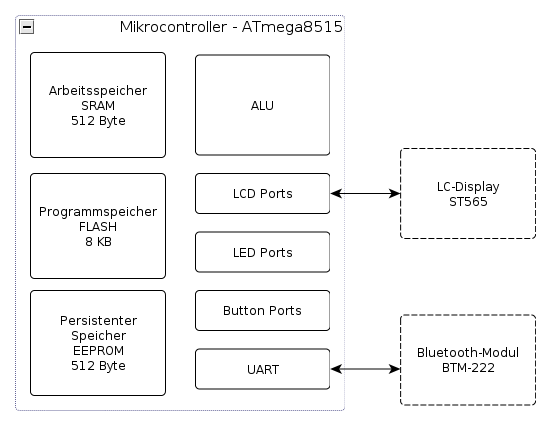
\includegraphics[width=0.7\textwidth]{media/letterbox-atmega-arch}
\end{center} \end{figure}

Die einzelnen Bauteile kommunizieren über einen 8-Bit-Datenbus. Besonders
auffällig ist, dass der ATmega8515 eine Harvard-Architektur darstellt. Im
Gegensatz zu einem Von-Neumann-Rechner liegen in einer Harvard-Architektur
Daten und Programm in unterschiedlichen Speichern. Die Programme liegen im
vergleichsweise großzügig bemessenen Programmspeicher (Flash), die
Programmdaten, der Stack und der Heap teilen sich den mit 512 Byte knapp
bemessenen Datenspeicher (SRAM). Für die persistente Speicherung von Daten über
Zeiten ohne Stromzufuhr hinweg existiert ein dritter persistenter Speicher
(EEPROM). Auch im EEPROM kann man nur 512 Byte speichern.

Der BTM-222-Baustein dient der Bluetooth-Kommunikation und arbeitet als Black-Box.
Beispielsweise nimmt der Baustein bei entsprechender Konfiguration automatisch
Verbindungen an. Der BTM-222 ist über eine serielle Schnittstelle ansprechbar.
Die Schnittstelle dient zur Übertragung von Nachrichtentext und
der Meldung von eingehenden Verbindungen. Man kann allerdings auch vom
Mikrokontroller aus über die serielle Schnittstelle AT-Befehle an den
BTM-222 übergeben.

\subsection{Software-Architektur des Briefkastens}

Auf der Hardware des Briefkastens läuft ein C-Programm, das aus verschiedenen,
handlichen Modulen zusammen gesetzt ist. Ein Schaubild illustriert den Zweck,
die verschiedenen Abstraktionsebenen und das Zusammenspiel der einzelnen
Module.

\begin{figure}[h!] \begin{center}
    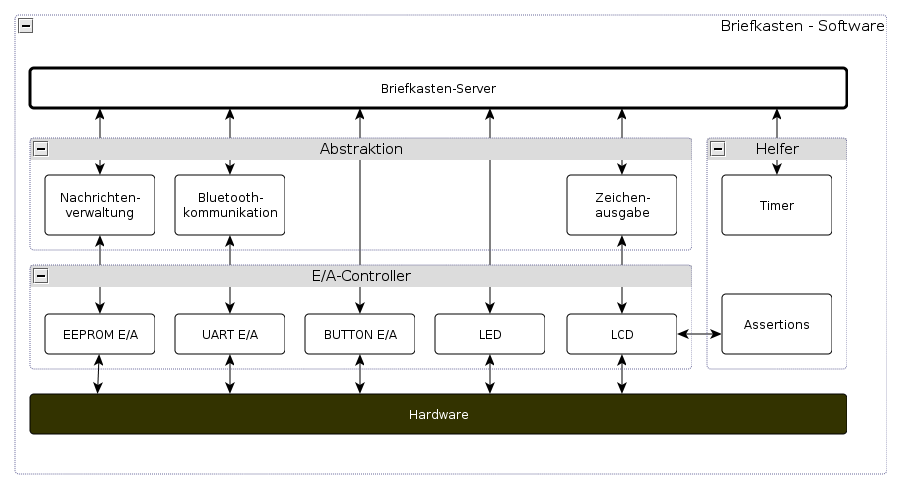
\includegraphics[width=\textwidth]{media/letterbox-arch}
\end{center} \end{figure}

Direkt über der Hardware liegen die E/A-Controller. Das sind Module, die alle
Formen von Eingabe und Ausgabe steuern und von der tatsächlichen Hardware
abstrahieren. Über den E/A-Controllern existieren Module, die für Abstraktion
sorgen, die über die einfachen Aufgaben der E/A-Controller hinausgeht. Für
manche Module, wie z.B. die Controller der Tasten oder Leuchtdioden ist eine
weitere Abstraktion nicht notwendig. Ganz oben liegt das Serverprogramm des
Briefkastens, das sich auch eines Timers bedient. Für Zwecke des Debuggings
besteht ein Assertion-Modul, das mangels besserer Ausgabemöglichkeiten vom LCD
abhängig ist.


\subsection{Software-Architektur des Mobiltelefons}

Die Applikation für das Mobiltelefon ist plattformunabhängig um auf
Betriebssystemen und Mobiltelefonen ganz verschiedener Hersteller zu laufen. Sie
ist in Java implementiert und baut auf drei Spezifikationen auf. Wie diese
implementiert sind, interessiert uns nicht weiter.

\begin{figure}[h!] \begin{center}
    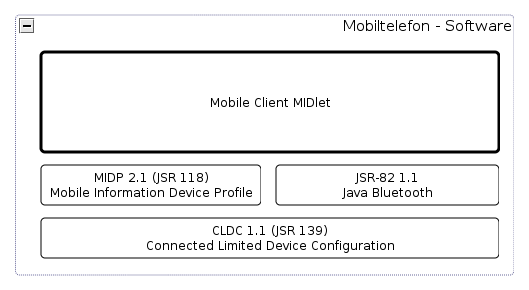
\includegraphics[width=0.7\textwidth]{media/mobile-client-arch}
\end{center} \end{figure}

Die Installation der Applikation erfolgt je nach Handy-Hersteller
unterschiedlich. Auf den meisten Geräten lässt sich die Applikation sehr
einfach installieren, in dem man sie z.B. über Bluetooth an das Handy schickt.


\section{Briefkasten}

Die gesamte Software auf dem Briefkasten ist in C programmiert. Änderungen am
Code sollen sich möglichst nur lokal auswirken. Das Finden und Ausbessern von
Schwachstellen wird dadurch erleichtert, dass das Programm in einzelne Module
mit unterschiedlichen Verantwortlichkeiten aufgeteilt ist.

\begin{tabular}{|l|l|}
    \hline
    {\bf Modul} & {\bf Pfad} \\
    \hline
    \hline
    EEPROM E/A & {\tt letterbox/eeprom/eeprom.h} \\
    \hline
    UART E/A & {\tt letterbox/uart/uart.h} \\
    \hline
    BUTTON E/A & {\tt letterbox/buttons/buttons.h} \\
    \hline
    LED & {\tt letterbox/buttons/led.h} \\
    \hline
    LCD & {\tt letterbox/lcd/lcd.h} \\
    \hline
    Zeichenausgabe & {\tt letterbox/lcd/text.h} \\
    \hline
    Bluetooth-Kommunikation & {\tt letterbox/uart/bt.h} \\
    \hline
    Nachrichtenverwaltung & {\tt letterbox/message/message.h} \\
    \hline
    Assertions & {\tt letterbox/assert/assert.h} \\
    \hline
    Timer & {\tt letterbox/timer/timer.h} \\
    \hline
    Server & {\tt letterbox/main.c} \\
    \hline
\end{tabular}


\subsection{Technische Anforderungen}

\subsection{Arbeitsspeicher}

Der Arbeitsspeicher (SRAM) des Mikrocontrollers ist auf 512 Byte beschränkt.
Dies entspricht 512 ASCII-Zeichen, was für ein System, das mit Textnachrichten
umgeht, nicht gerade viel ist. So hat sich letztendlich der Arbeitsspeicher als
größte Hardwareeinschränkung ergeben, weit vor der Taktrate, die mit 16 MHz
überaus großzügig bemessen war. Wir haben darauf geachtet, dass der Code
möglichst effizient ist, wobei wir jedoch den Fokus - soweit es ging - auf klaren,
verständlichen Code gelegt haben.

Jedoch mussten wir einige Abstriche machen, um Speicher zu sparen. So ist
es trotz unseres zeilenbasierten Übertragungsprotokolls nicht möglich, eine
Zeile Text direkt vom UART in den Arbeitsspeicher einzulesen, da die
eingelesene Zeile kein Längenlimit hat, unser Arbeitsspeicher jedoch schnell
an seine Grenzen kommt. Daher werden eingehende Zeilen direkt in den EEPROM
geschrieben.

\subsection{Robustheit}

Eingebettete Systeme haben hohe Anforderungen, was die Zuverlässigkeit
der Programme anbelangt. Besonders sorgfältig muss die Kommunikation
zwischen Briefkasten und dem Mobilgerät ablaufen.

Zu dem C-Programm müssen wir ehrlicherweise anmerken, dass wir uns nicht
besonders um programmweite Konsistenz bei den verwendeten Datentypen
ge\-kümmert haben. Im Folgenden kommen nun die Modulbeschreibungen. Sie
enthalten je eine Übersicht der deklarierten Prozeduren um einen Zusammenhang
zur tatsächlichen Implementierung herzustellen.


\subsection{E/A-Controller}

Die E/A-Controller sind dafür zuständig, die Hardware auf der Ebene von Bits
und Bytes zu steuern. Zu ihren Aufgaben gehört das Auslesen der Tasten, das An-
und Ausknipsen der Leuchtdioden,  das Beschreiben des Speichers, die
Ansteuerung des LC-Displays und letztendlich die Kommunikation über die
serielle Schnittstelle mit dem Bluetooth-Modul. Sie sind sozusagen die Treiber
für das Server-System.

\subsubsection{EEPROM}

Das EEPROM-Modul stellt eine einfache Schnittstelle für Lese- und
Schreibzugriffe auf den persistenten Speicher bereit:
 
\lstinputlisting{eeprom.h}

Bytes können im EEPROM einzeln addressiert werden. Die Implementierung ist
direkt aus der Referenzdokumentation entnommen.

Wir haben uns im gesamten Projekt bemüht, die Zahl der Lese- und
Schreibzugriffe auf das EEPROM zu minimieren und wann immer möglich, nur mit
Daten aus dem flüchtigen Arbeitsspeicher zu arbeiten.

\subsubsection{UART}

Die Kommunikation zwischen dem Briefkasten und dem Bluetooth-Bauteil erfolgt
über eine serielle Schnittstelle. Diese serielle Schnittstelle wird von
einem UART-Baustein implementiert. Für die Steuerung des UART-Bausteins haben
wir  Peter Fleurys UART-Library benutzt, die wiederum auf dem UART-Beispielcode 
von Atmel basiert. Die Library bietet Unterstützung für die Ansteuerung zweier
separater UART-Bausteine, daher gibt es in der Bibliothek für jede Funktion
zwei Versionen. Unser Mikrocontroller hat jedoch nur einen UART, sodass ein
Teil der Funktionen ungenutzt sind. Dieser Code ist streng genommen redundant,
wir haben uns jedoch entschieden, keine eigenen Änderungen an der Library
vorzunehmen, um eventuelle zukünfige Updates einfach zu halten.

Das UART-Modul stellt die folgenden Prozeduren bereit:

\lstinputlisting{uart.h}

Die UART-Library ermöglicht das nichtblockierende Lesen von einzelnen Bytes,
sowie das Schreiben von Bytes oder ganzer Bytefolgen. Eine Unterstützung für
das Lesen von ganzen Strings, wie etwa einzelnen Zeilen, bietet diese Komponente
nicht -- diese Funktionalität wurde in der Bluetooth-Komponente selbst implementiert.

Wichtig bei der Benutzung der seriellen Schnittstelle ist die korrekte Konfiguration.
Die Baudrate, also die Geschwindigkeit, mit der Symbole pro Sekunde über die Leitung
geschickt werden, muss korrekt eingestellt sein. Ebenso muss darauf geachtet werden, ob
ein Paritätsbit gesendet wird oder nicht.

\subsubsection{Tasten}

Das BUTTONS-Modul stellt die folgenden Prozeduren bereit:

\lstinputlisting{buttons.h}

Das Modul stellt nur die Möglichkeit bereit, abzufragen, ob und welcher Button gedrückt ist.
Die Interaktion mit dem Benutzer wird nicht über Interrupts geregelt, sondern geht 
ausschließlich über regelmäßiges Abfragen. Die Hardware des Briefkastens verfügt über zwölf Tasten.
Eine Abfrage liefert einen Rückgabewert von 1 bis 12 zurück, der spezifiziert,
welche Taste gedrückt wurde. Auch diese Funktion blockiert nicht, daher
wird 0 zurückgegeben, falls keine Taste gedrückt wurde.

Nur die vier Tasten direkt unterhalb des Displays finden Verwendung -- 
die verbleibenden acht Tasten auf dem Boards dienen keinem Zweck..

\subsubsection{Leuchtdioden}

Das LED-Modul stellt die folgenden Prozeduren bereit:

\lstinputlisting{led.h}

Das LED-Modul ist, wie sich das für Mikrocontroller fast schon gehört, als
erstes entstanden, um überhaupt herauszubekommen wie die Interaktion mit
der Hardware abläuft. Das Board enthält drei LEDs: eine rote, eine grüne
sowie eine blaue, die links neben dem Display angebracht sind.

Die LEDs waren im Laufe des Projektes hauptsächlich für Debugging-Zwecke
dienlich, da die Unterstützung des Displays erst relativ spät hinzugefügt
wurde. So konnten durch das Blinken der LEDs auf einfache Weise kleine
Integerwerte, wie etwa der aktuell gedrückte Button dargestellt werden.

Das fertige Projekt nutzt die LEDs nur noch für Statusinformationen
wie den Verbindungsaufbau oder das Vorhandensein neuer Nachrichten.

\subsubsection{Flüssigkristallanzeige}

Das LCD-Modul stellt die folgenden Prozeduren bereit:

\lstinputlisting{lcd.h}


\subsection{Abstraktion}

In einer Abstraktionsschicht, die sich nur noch kaum direkt mit Bits und Bytes
auseinandersetzen muss, befinden sich die Module für die Nachrichtenverwaltung,
für die Kommunikation mit Bluetooth-Klienten und für die Ausgabe von Text auf
der Anzeige.


\subsubsection{Nachrichtenverwaltung}

Die Nachrichtenverwaltung kümmert sich um das Auslesen, Speichern und
Löschen der empfangenen Nachrichten. Die Nachrichteninhalte sind im EEPROM
gespeichert.  Da die Nachrichten zwar in geordneter Reihenfolge beim
Briefkasten eingehen, diese aber vom Empfänger in beliebiger Reihenfolge
gelöscht werden können, liegt über dem EEPROM-Speicher noch eine
In\-di\-rek\-tions\-schicht. Der EEPROM-Speicher wird von der
Nachrichtenverwaltung in verschiedene Blöcke aufgeteilt, und zwar in
sogenannte \textit{Nachrichtenblöcke} und einen sogenannten
\textit{Superblock}.

% \begin{tabular}{|l|l|l|l|}
%     \hline
%     {\bf Datum} &{\bf Format} & {\bf Speicherort} & {\bf Bezeichnung} \\
%     \hline
%     \hline
%     Nummer & {\tt uint8\_t} & Superblock & {\tt msg\_num} \\
%     \hline
%     Status & {\tt char} & Nachrichtenblock & {\tt ---} \\
%     \hline
%     Text & 120 x {\tt char} & Nachrichtenblock & {\tt text} \\
%     \hline
% \end{tabular}

\begin{tabular}{|l|l|l|l|}
    \hline
    {\bf Adresse} & {\bf Datum} & {\bf Format} & {\bf Beschreibung} \\
    \hline
    \hline
    0 & Status & {\tt char} & {\tt STATE\_EMPTY, STATE\_NEW,  STATE\_READ} \\
                          &&& Für zukünftige Erweiterungen. \\
    \hline
    1-7 & Reserviert & {\bf --- }  & Reserviert für zukünftige Erweiterungen. \\
    \hline
    8-119 & Text & 120 x {\tt char} & Text der Nachricht. Durch ein \\
                                  &&& Null-Byte wird das vorzeitige \\
                                  &&& Ende einer Nachricht gekennzeichnet. \\
    \hline
\end{tabular}

Der Text und der Status der Nachrichten sind in Nachrichtenblöcken zu je 120
Byte gespeichert. Der Grund, dass die Größe keiner Zweierpotenz entspricht,
liegt an der geringen Größe des EEPROM-Speichers. In den 512 Bytes dieses
Speichers muss auch noch der Superblock Platz finden. Das Limit der
Nachrichtenlänge auf 112 Bytes ersparte uns auch die Implementierung einer
Scrollfunktion, damit die Nachricht auch dann gelesen werden kann, wenn sie
nicht ganz auf die Anzeige passt. Das hätte natürlich ein schönes Feature
dargestellt.

Der Superblock besteht aus \textit{Blockzeigern} und einem
\textit{Nachrichtenzähler}, der angibt, wie viele Nachrichten momentan auf dem
Briefkasten gespeichert sind. Die Blockzeiger bilden
\textit{Nachrichtennummern} auf Nachrichtenblöcke ab.

\begin{figure}[h!] \begin{center}
    \includegraphics[width=0.7\textwidth]{media/eeprom}
\end{center} \end{figure}

Wird vom Briefkasten eine neue Nachricht  empfangen, und ist noch Platz für
diese Nachricht, so wird der Nachrichtentext in einen freien Block geschrieben,
ein Blockzeiger auf diesen Block angelegt und der Nachrichtenzähler erhöht. Die
neue Nachricht erhält die größte Nummer. 

Löscht der Empfänger eine Nachricht, so wird der zugehörige Blockzeiger
entfernt. Die Nummern aller neueren Nachrichten werden dekrementiert, die
Blockzeiger rücken auf (eine verkettete Liste würde diese Prozedur ersparen).
Zuletzt wird der Nachrichtenzähler erniedrigt.

Dieses Prinzip führt dazu, dass sich die zeitliche Ordnung der Nachrichten
stets in den ihnen zugewiesenen Nummern wiederspiegelt, und dass bei
Löschvorgängen sehr wenig Arbeit zu verrichten ist. Die Nachrichten auf dem
EEPROM werden nicht wirklich gelöscht, die Blöcke werden freigegeben, indem die
Blockzeiger entfernt werden.

Die Nachrichtenverwaltung bedient sich verschiedener Techniken, um den
Anforderungen gerecht zu werden. Sie stellt ein Streaming-Interface zum
Schreiben und Lesen von Nachrichten bereit, um den Einsatz von Puffern
überflüssig zu machen. Damit können Schreib- und Lesevorgänge sehr effizient
ablaufen.

Um die nötigen Schreib- und Lesezugriffe auf den EEPROM-Speicher zu begrenzen,
wird der Superblock im Arbeitsspeicher zwischengespeichert und nur beim Löschen
und beim Speichern einer Nachricht wird der Superblock in den EEPROM
zurückgeschrieben. Die Ersparnis der Lesezugriffe ist offensichtlich, die der
Schreibzugriffe jedoch nicht: Das Aufrücken der Blockzeiger soll nicht direkt
auf dem EEPROM geschehen, sondern im Arbeitsspeicher.

Die Nachrichtenverwaltung ist so ausgelegt, dass sie auch mit einem korruptem
Superblock umgehen kann. Dies ist extrem wichtig. Man stelle sich vor, durch
einen Stromausfall, ein sonstiges unerwartetes Ereignis oder durch ein erneutes
Flashen der Software wird der Superblock korrumpiert.  Das kann direkt dazu
führen, dass der Briefkasten sich nicht mehr starten lässt. Bei Programmstart
wird der Superblock in den Arbeitsspeicher kopiert.  Nun könnte durch den
korrupten Superblock der Nachrichtenzähler negativ sein was das Programm unter
Umständen in eine Endlosschleife geraten lässt. Oder die Blockzeiger führen ins
Nirvana. Ebenso könnten zwei Blockzeiger auf den gleichen Nachrichtenblock
zeigen. Auf all diese Fälle wird beim Einlesen des Superblocks geprüft und im
Fehlerfall wird der Superblock in einen validen Nullzustand überführt.

Für die Nachrichtenverwaltung existieren gründliche automatische Tests.  Damit
diese Tests auf jedem Rechner laufen - und nicht nur auf dem AVR - kommt ein
gemocktes EEPROM-Modul zum Einsatz.

Das Message-Modul exportiert die folgenden Funktionen:

\lstinputlisting{message.h}


\subsubsection{Bluetooth-Kommunikation}

Das Bluetooth-Modul stellt die folgenden Prozeduren bereit:

\lstinputlisting{bt.h}


\subsubsection{Zeichenausgabe}

Das Modul zur Zeichenausgabe ermöglicht die Ausgabe von Text auf der
Flüs\-sig\-kris\-tall\-an\-zei\-ge. Es kümmert sich um die Umwandlung eines
Zeichens ({\tt char}) in eine darstellbare Bitmatrix und sorgt für einen
automatischen Zeilenumbruch. Maskierungen erlauben es, dass die Textausgabe
invertiert erfolgt (weiß auf schwarz). Das LC-Display unterstützt von sich aus
keine Zeichenausgabe. Deshalb haben wir einen eigenen Zeichensatz entworfen,
der auf die Größe und Auflösung des LC-Displays angepasst ist. Der Zeichensatz
umschließt alphanumerische Zeichen und einige Satzzeichen, erhebt aber keinen
Anspruch auf Vollständigkeit.

Ein Buchstabe wird durch eine 8x5-Bit-Matrix repräsentiert. Die
Spaltenvektoren werden in je einem Byte gespeichert. Das oberste Bit
entspricht dem höchstwertigen Bit. Eine 1 entspricht einem schwarzen
Bildpunkt, die 0 einem weißen Bildpunkt. Mit der XOR-Maske {\tt 0xff} lässt
sich so ein Schwarz-auf-Weiß-Buchstabe auf einfache Art und Weise
invertieren. Diese Technik wird beim Zeichnen von Dialogen und Bedienelementen 
verwendet. Die Speicherung der Spaltenvektoren bietet sich auf an,
da die Ausgabe an den LC-Display sowieso schon Spalte für Spalte erfolgt.

\begin{figure}[h!] \begin{center}
    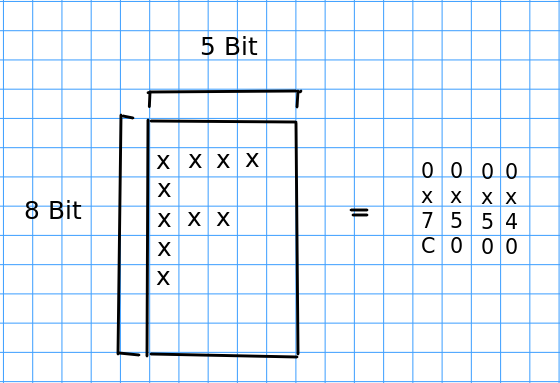
\includegraphics[width=0.7\textwidth]{media/char}
\end{center} \end{figure}

Mit diesem Format benötigt jedes Zeichen genau 5 Byte. Der Zeichensatz enthält
über 45 Zeichen, womit er insgesamt über 225 Byte an Speicherplatz benötigt.
Damit im Arbeitsspeicher kein wertvoller Platz  verschwendet wird, ist der
Zeichensatz mit der {\tt pgmspace}-Erweiterung des GCC in den Programmspeicher
ausgelagert.

Das Zeichenausgabe-Modul stellt die folgenden Prozeduren bereit:

\lstinputlisting{text.h}


\subsection{Helfer}


\subsubsection{Timer}

Eine robuste Kommunikation ist ohne Timeouts nicht vorstellbar, jedoch ist die
Timeout-Behandlung sehr lowlevel, daher haben wir einen Wrapper geschrieben um
uns das Leben einfacher zu machen.  Das Timer-Modul bietet die Möglichkeit auf
einfachere Art mit Timeouts zu arbeiten. Dazu wird zuallererst eine gewünschte
Zeitspanne in \texttt{timer\_start} definiert. Danach kann der Nutzer
\texttt{timer\_poll} aufrufen um herauszufinden ob diese Zeitspanne bereits
überschritten wurde oder noch nicht. Intern benutzen wir den Quarz und setzen
die Timer-Skalierung des Mikrocontrollers auf den Maximalwert 1024 und prüfen
ob der Timer einen bestimmten, errechneten Wert überschritten hat -- sobald
dies der Fall ist, kann dem User ein abgelaufenes Timeout signalisiert werden.

Das Timer-Modul stellt die folgenden Prozeduren bereit:

\lstinputlisting{timer.h}


\subsubsection{Assertions}

Das Assertion-Modul ist eine nützliche Methode zum Debuggen.  Der
problematische Teil ist die Ausgabe einer Nachricht, falls eine Assertion nicht
zutrifft. Derzeit sind die Assertions von der LC-Anzeige und deren Steuerung
abhängig. Das Assertion-Modul stellt die folgenden Prozeduren bereit:

\lstinputlisting{assert.h}


\subsection{Server}

Der Server ist das Hauptmodul, das alle anderen Module benutzt. Er erledigt
drei Aufgaben, das Empfangen von Nachrichten, die Verarbeitung der
Benutzeranfragen und die Steuerung der Bedienungsoberfläche. Der Server
arbeitet in einer hier natürlich erwünschten Endlosschleife. Aus Sicht des
Servers gibt es keinerlei Interrupts. Tatsächlich verwenden die UART-Funktionen
Interrupts, wovon der Server allerdings nichts mitbekommt und sich deshalb auf
das re\-gel\-mä\-ßige, zyklische Abfragen von Zuständen beschränkt.

Zum Empfangen einer Nachricht wartet der Server auf eine über die serielle
Schnittstelle eingehende 'CONNECT XYZ'-Nachricht. Das Lesen der eingehenden
Daten erfolgt über das Bluetooth-Modul. Nach Aufbau der Verbindung wartet der
Server ein bestimmtes Zeitfenster auf die Nachricht. Die eingehende Nachricht
wird direkt über die Nachrichtenverwaltung ind das EEPROM ge\-schrie\-ben. In
beiden Fällen, ob nun eine Nachricht kommt oder nicht - wird die
Bluetooth-Verbindung nach diesem Zeitfenster bzw. nach dem Lesen einer Zeile
(mit Limit!) durch den Server mit einem AT-Kommando an den BTM-222 beendet.
Dieses Vorgehen sorgt für eine stabilen Server, der auch durch Fehlverhalten
oder Absicht des Clients nicht angreifbar ist. Eine Denial-of-Service-Attacke
ist natürlich immer noch möglich.

Das Senden einer Empfangsbestätigung ist bisher nicht implementiert. Der Client
muss sich also mit dem Prinzip `fire and forget' begnügen.

Zwischen den Abfragen, ob eine neue Verbindung angenommen wurde, bearbeitet der
Server Anfragen des Benutzers. Ist eine Taste gedrückt, so wird die
entsprechende Aktion ausgelöst und gewartet, bis die Taste wieder losgelassen
wurde.

Der Server steuert auch die Bedienungsoberfläche. Dabei unterstützt er das
Anzeigen von modalen Dialogen, die in bestimmten Fällen auch vom Benutzer
geschlossen werden können. Diese Dialoge bestehen aus Text, der die gesamte
Anzeige füllt. Da diese Texte viel Speicher im SRAM benötigen, sind sie in den
Programmspeicher ausgelagert. Um deren benötigten Speicherplatz
ein\-zu\-schrän\-ken könnte man sie noch komprimieren, in dem man Leerzeilen
mit entsprechendem Linefeed kodiert anstelle der expliziten Form mit
Leerzeichen. Davon haben wir allerdings mangels Notwendigkeit abgesehen.

Um die Knöpfe auf der Anzeige und die Dialoge in weißer Schrift auf
schwarzem Hintergrund zu zeichnen, verwendet der Server die Möglichkeit
des LCD-Moduls die Ausgabe zu maskieren. Die LC-Anzeige wird also nicht
invertiert, sondern nur die Daten, die an die LC-Anzeige gehen.

Das Server-Modul ist in die folgenden, privaten Prozeduren unterteilt:
\lstinputlisting{main.c}


\section{Mobiltelefon}

Die Client-Anwendung auf dem Mobiltelefon ist in Java geschrieben. Sie baut auf
drei Spezifikationen auf. Zum einen auf dem CDLC (Connected Limited Device
Profile), das die grundlegenden Klassen der Standardbibliothek und die
unterstützte Sprachfunktionalität auf den mobilen Geräten festlegt. Des
weiteren benötigt die Anwendung noch eine Möglichkeit, eine graphische
Benutzeroberfläche darzustellen. Dies liefert das MIDP (Mobile Information
Device Profile). Zu allerletzt ist der Zugriff auf den Bluetooth-Stack im
Mobiltelefon notwendig.  Dafür sorgt die JSR-82-Spezifikation. Insgesamt ist
das eine typische Umgebung für die Entwicklung einer Java-Anwendung. Man
programmiert gegen eine Menge von Schnittstellen an und kümmert sich nicht um
die spätere Implementierung.

Die Client-Anwendung auf dem Mobiltelefon hat grundsätzlich zwei Aufgaben, zum
einen die Kommunikation mit dem Benutzer, zum anderen die Suche nach
Bluetooth-Geräten. Damit der Benutzer nicht lange auf das Ende der Gerätesuche
warten muss, wird die Suche direkt bei Programmstart in einem eigenen Thread
gestartet. Dies war eine kleine Herausforderung, da wir uns bei der Entwicklung
der Anwendung nun mit drei verschiedenen Threads beschäftigen mussten.

Die Benutzerführung soll so einfach wie möglich gestrickt sein. Bevor der
Em\-pfänger ausgewählt werden kann, muss natürlich auf den Abschluss der
Ge\-rä\-te\-suche gewartet werden, falls dies bis dahin noch nicht erfolgt ist.

\begin{figure}[h!] \begin{center}
    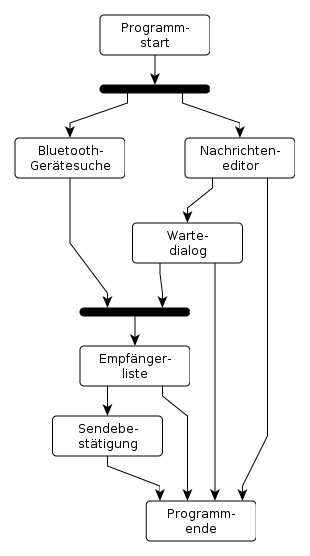
\includegraphics[width=0.4\textwidth]{media/mobile-client-flow}
\end{center} \end{figure}

Die Anwendung ist in folgende Klassen untergliedert:

\begin{tabular}{|l|l|}
    \hline
    {\bf Klasse} & {\bf Superklasse} \\
    \hline
    {\tt CarrierpigeonMIDlet} & {\tt javax.microedition.midlet.MIDlet} \\
    \hline
    {\tt MessagePanel} & {\tt javax.microedition.lcdui.Form} \\
    \hline
    {\tt WaitPanel} & {\tt javax.microedition.lcdui.Form} \\
    \hline
    {\tt SendPanel} & {\tt javax.microedition.lcdui.List} \\
    \hline
    {\tt ErrorPanel} & {\tt javax.microedition.lcdui.Form} \\
    \hline
    {\tt DeviceDetector} & {\tt java.lang.Object}\\
    \hline
    {\tt DefaultDeviceDetector} & {\tt DeviceDetector} \\
    \hline
    {\tt MockDeviceDetector} & {\tt DeviceDetector} \\
    \hline
\end{tabular}

Im Nachrichteneditor ({\tt MessagePanel}) kann der Benutzer eine Nachricht
eintippen.  In der Regel bietet das Mobiltelefon dabei automatisch eine
Schreibhilfe mit T9. Drückt man als Benutzer auf Senden, so erscheint unter
Umständen ein Wartedialog ({\tt WaitPanel}) bis die  Gerätesuche beendet ist.
Eine Filterung der gefundenen Geräte erfolgt nicht, dem Benutzer wird also eine
Liste von sichtbaren Geräten in seinem Umfeld präsentiert ({\tt SendPanel}), in
der ein Empfänger ausgewählt werden kann. Nach dem Senden der Nachricht wird
eine Sen\-de\-be\-stä\-ti\-gung angezeigt (keine Empfangsbestätigung).

Die Gerätesuche erfolgt mittels einem Observer-Pattern und der Klasse \\{\tt
javax.bluetooth.DiscoveryAgent}.  Dabei haben wir sorgfältig auf korrektes
Multi-Threading geachtet, und die beteiligten Klassen entsprechend
synchronisiert, insbesondere um Race-Conditions zu vermeiden. Eine solche
Race-Condi\-tion könnte z.B. in {\tt DefaultDeviceDetector.waitForCompletion}
auftreten, die dazu führt, dass das Mobiltelefon ewig den Wartedialog anzeigt,
obwohl die Suche tatsächlich schon abgeschlossen ist. Die in der obigen
Illustration sichtbare Barriere wird mit der Kombination aus {\tt wait} und
{\tt notifyAll} erreicht. Die sonst übliche Technik mit {\tt Thread.join} hat
sich hier nicht angeboten.

Wie auch in Java Swing verwendet auch die Oberfläche auf dem Mobiltelefon zwei
verschiedene Threads. Bei Swing ist das der \textit{Event-Dispatching-Thread}
und der \textit{Realizing Thread}.  Bei MIDP funktioniert das analog. Die
MIDP-Spezifikation zeigt, dass man mit {\tt Display.callSerially} Aufgaben in
die Warteschlange des Event-Dispatching-Threads einreihen kann. Diese
Möglichkeit haben wir intensiv genutzt, um eine korrekte Bedienungsoberfläche
mit schnellen Antwortzeiten zu implementieren.

Die Anwendung besitzt leider keine automatischen Tests. Dafür allerdings
unterstützt sie das manuelle Testen in einer simulierten Umgebung. Mit
dem {\tt MockDeviceDetector} kann das Programm im Simulator ohne
einer echten Ge\-rä\-te\-suche und echten Bluetooth-Verbindungen laufen.

\section{Projektumgebung}

\subsection{Zusammenarbeit}

Das Projekt ist bei bitbucket.org registriert, wo wir unser Open-Source-Projekt
entgeltfrei in einem Mercurial-Repository liegen haben. Vielen Dank an dieser
Stelle!  Mercurial hat sich als sehr gute Wahl herausgestellt. Als verteiltes
Versionierungssystem glänzte es besonders, wenn wir uns mal wieder in Räumen
oder Zügen ohne Internetanschluss bewegten oder gelegentlich ohne größere
Absprachen treffen zu müssen, an den gleichen Dateien arbeiteten.

Bei der Entwicklung saßen wir in der Regel mindestens zu zweit an jeder
Aufgabe, was zu der erfreulichen Tatsache geführt hat, dass es kaum zu solchen
Situationen gekommen ist, in denen \textit{keiner} von zwei Leuten wusste,
warum eine bestimmte Funktion wie programmiert worden ist. Die Verteilung des
Wissens über die Entwickler war deshalb nahezu optimal.

\subsection{Werkzeuge}

Die Programmierung erfolgte auf handelsüblichen Notebooks, die dazu benötigten
Build-Skripte und Werkzeuge sind auf den meisten Betriebssystemen zu bekommen.
Das Serverprogramm für den Briefkasten kann mit dem AVR-GCC (wir haben die
Versionen 4.3 und 4.4 verwendet) und der avr-libc
prinzipiell unter jedem Betriebssystem kompiliert werden. Das Aufspielen der
kompilierten Software geschieht über \texttt{avrdude} und ab diesem Zeitpunkt ist das
Gerät unabhängig vom Notebook.

Die Software ist in C99 geschrieben, nutzt aber spezielle Erweiterungen des
AVR-GCC, sodass die Portierbarkeit in dieser Hinsicht eingeschränkt ist. Dies
scheint aber kein großes Problem zu sein, da der GCC sich in der Community der
AVR-Programmierer als ein Standardtool etabliert hat.

    \begin{tabular}{|r||l|}
        \hline
        Hardware & ATmega 8515, BTM-222, ST7565 LCD, AVRISP2 \\
        \hline
        Languages & C, Java, Python\\
        \hline
        Framework & Java Micro Edition, Peter Fleury's UART library\\
        \hline
        Compilation & {\tt avr-gcc, avr-objcopy, avr-strip, avrdude,} \\
                    & {\tt avr-nm, avr-size, splint, python, ant} \\
        \hline
        Helpers & {\tt hcitool, rfcomm, gtkterm, jpnevulator} \\
        \hline
    \end{tabular}



\section{Ausbaumöglichkeiten}

Wie immer gibt es eine Menge Möglichkeiten, die derzeitige Implementation zu
erweitern und verbessern. Wir listen hier einige Verbesserungsmöglichkeiten
auf:

\begin{description}
    \item[Scrollen durch den Nachrichtentext] Wenn genügend persistenter Speicher vorhanden wäre, könnte man 
        längere Nachrichten zulassen. Eine Scrollfunktion würde notwendig, ein nettes
        Feature.
    \item[Erweiterung des persistenten Speichers] 512 Byte reichen gerade so für vier Nachrichten. Für Test-
        und Demonstrationszwecke ist dies natürlich völlig ausreichend, eine Erweiterung wäre aber vielleicht
        technisch interessant.
    \item[Nachrichtenverwaltung mit verketteter Liste] Abschaffen des Superblocks und Einführung einer verketteten
        Liste, sowohl in der programminternen Darstellung im Arbeitsspeicher als auch in den Nachrichtenblöcken
        des EEPROMs. Das würde wohl zu einem natürlicheren und leichter ver\-ständ\-lichen Modell der 
        Nachrichtenverwaltung führen.
    \item[Empfangsbestätigung senden] Dem Mobiltelefon erhält eine Rückmeldung vom Briefkasten nach dem
        dieser die Nachricht erhalten hat. Damit lässt sich auch das Problem lösen, was zu tun ist, 
        wenn der Briefkasten voll ist.
    \item[Automatische Tests] Es ist uns gelungen, SimulAVR als AVR-Simulator mit dem GNU Debugger
        zu verbinden und dort auch das AVR-Programm auszuführen. Allerdings hatten wir Probleme mit
        der Simulation des EEPROMs und haben diesen Faden nicht weiter verfolgt. Auch die Möglichkeiten
        zum Testen der Anwendung des Mobiltelefon haben wir nicht ausgeschöpft.
    \item[Vervollständigung des Zeichensatzes] Bisher sind mehr als 45 Zeichen darstellbar. Nachdem im
        Programmspeicher noch einiger Platz verfügbar ist, könnte man den Zeichensatz auf Umlaute
        und andere Sonderzeichen erweitern.
    \item[Korrektes Encoding auf dem Mobiltelefon] Momentan gibt es bei dem Programm auf dem Mobiltelefon
        die typischen Probleme mit Umlauten. Das Eingabetextfeld ist auf 112 Zeichen beschränkt. Das
        Mobiltelefon sendet aber zwei Bytes für einen Umlaut (UTF-8).
    \item[Einsatz der Leuchtdioden] Kosmetisches Feature. Implementierung mit derzeitigem zyklischen Servermodell
        ist allerdings nicht ganz trivial. Eine Lösung wäre die Verwendung der Technik des Timers, um z.B.
        Blinken der LEDs während des Empfangens einer Nachricht zu ermöglichen.
    \item[Filterung der Geräte] Auf dem Mobiltelefon werden derzeit alle Bluetooth-Geräte aufgelistet. Schön
        wäre es hier, wenn nur die Geräte angezeigt werden, die das entsprechende Nachrichtenprotokoll
	sprechen.
\end{description}


%\begin{tabular}{|l|l|l|}Zeilen Worte  Bytes
%614    1782   19744
%2595    8945   71127
%\newpage
%
\appendix

\newpage

% include sources that are not cited explicitly
% \nocite{}

% http://java.sun.com/products/jfc/tsc/articles/threads/threads1.html

\bibliographystyle{plain}
\bibliography{article} 

\end{document}
